
Q-learning base algorithm shows the iterative update rule for an action value function, which is said to find optimality for any FMDP assuming infinite exploration.


$Q^{n e w}\left(s_{t}, a_{t}\right) \leftarrow(1-\alpha) \cdot \underbrace{Q\left(s_{t}, a_{t}\right)}_{\text {old value }}+\underbrace{\alpha}_{\text {learning rate }} \cdot \overbrace{(\underbrace{r_{t}}_{\text {reward }} +  \underbrace{\gamma}_{\text {discount factor }}\cdot \underbrace{\max_{a}Q\left(s_{t+1}, a\right))}_{\text{estimate of optimal future value}}}^{\text {learned value }}$

\noindent
With learning rate $\alpha$, reward $r_t$ for moving into $s_{t+1}$ from $s_t$ taking action $a$ and the discount factor $\gamma$, which controls how important the future rewards are, or how much into the future the model looks.\\

\noindent
On top of the basic algorithm, DQN is a functional approximation variant of the Q-learning, in which the model is supposed to be deep (more than one layer). We used a delayed network (updated every 20 episodes) to compute the delayed values and tried both GLIE epsilone-greedy as well as a linear decaying epsilone of the form of $\frac{5mil-SF}{5mil}$, with $SF$ being the total number of frames out of all episodes, and capped the it's minimum epsilon value to $\epsilon=0.1$. We noticed that having the model around episode 50k with about $50\%$ win-rate and $\epsilon=0.1$ actually worsened the model from that point onwards, so we capped $\epsilon$ to 0.3 untill episode 125000 and have it linearly decrease until 180000 (where it reached 0.1).\\


\noindent
Figure 2 shows the two main data augmentation/preprocessing we ended up doing for the dqn models. Aside from that, we also tried stacking them on a 3rd dimension, like the channels of an RGB image and have according convolution layers, but it seemed a little bit worse than putting the images on top of each other. \\

\noindent
Vertically stacked images with downscaling and gray-scaling, as described also in the "Preprocessing Pipeline", section 3. The idea behind leaving the right pallet blacked out, came after we noticed that the model was doing decently against simple-ai (around $60\%$ win-rate), while having around $50\%$ against Karpathy. Rendering it, we noticed that that the dqn model probably learned that it's highes action-values, are those that get it's pole into the same position as the simple-ai model (it was probably imitating it), and the 60\% (so "better" than simple-ai) was probably a mere consequence of the delay with which it went to catch the ball, catching it with the edge, speeding it up and winning a little be more often.\\

    \begin{minted}{python}
            Conv2d(channels, 32, kernel_size=(7, 7), stride=1)
            MaxPool2d(kernel_size=(2, 2))
            Conv2d(32, 32, kernel_size=(5, 5), stride=1)
            MaxPool2d(kernel_size=(2, 2))
			Linear(9792, 120)
			Linear(120, 3)
	\end{minted}

\noindent
The model architecture that ended up being good enough to beat simple-ai on 80\%+, was composed of two convolution layers, with max-pooling layers in between, followed by two linear layers, $9792x120$ and $120x3$:






\begin{figure}[!htb]
    \centering
    \begin{subfigure}{.49\textwidth}
        \centering
        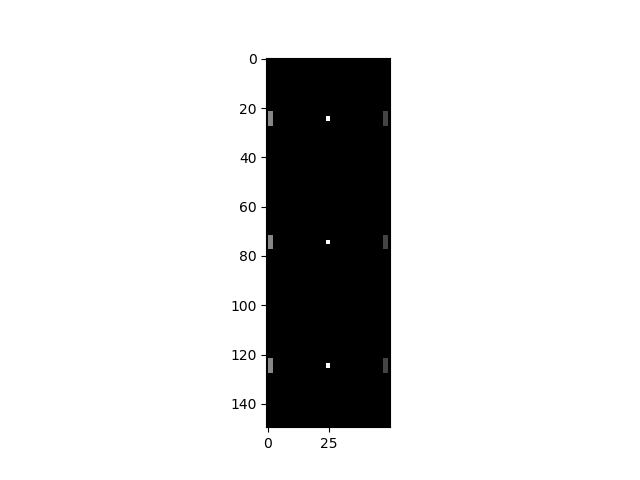
\includegraphics[width=\textwidth]{figures/dqn_training_image.png}
        \caption{Preprocessed 3-stacked images}
        \label{fig-raw}
    \end{subfigure}
    \begin{subfigure}{0.49\textwidth}
        \centering
        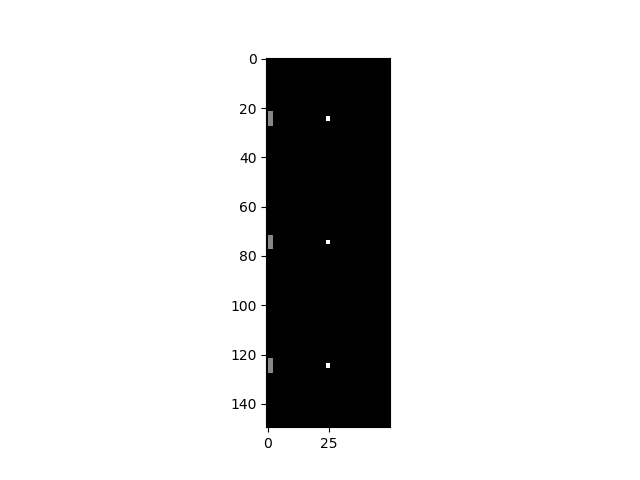
\includegraphics[width=\textwidth]{figures/dqn_training_image_blacked_out_pallet.png}
        \caption{Preprocessed 3-stacked images with blacked-out pallet}
        \label{fig-bw}
    \end{subfigure}
    \caption{DQN image augmentation and processing}
    \label{fig-small}
    \label{fig-process}
\end{figure}